% ===========================================================================
% fig-language-transfer.tex — per-language spontaneous localization F1,
% trained vs never-trained languages.
% BODY ONLY (tikzpicture). Wrapper/caption/label live in the section file.
% Requires % ===========================================================================
% fig-style.tex — shared colour / marker scheme for EVERY main-paper figure.
% \input this ONCE from the preamble of main.tex (after tikz + pgfplots).
%
% House rule: the palette is defined here and nowhere else. Each series also
% gets a distinct marker AND line style so the figures survive grayscale
% printing.
%
%   \sysname / deployed .. cSys   (blue!70!black)    mark *
%   opus / claude ........ cOpus  (red!70!black)     mark square*
%   gpt .................. cGpt   (teal!70!black)    mark triangle*
%   kimi ................. cKimi  (violet!70!black)  mark diamond*
%   flash ................ cFlash (orange!70!black)  mark pentagon*
%   greedy / baseline .... cBase  (gray)             mark o
% ===========================================================================
% The pipeline diagram needs the calc library for coordinate arithmetic; the
% rest of the libraries are already loaded in main.tex's preamble.
\usetikzlibrary{calc}
% Hatching, so bar charts stay readable in grayscale.
\usetikzlibrary{patterns}

\colorlet{cSys}{blue!70!black}
\colorlet{cOpus}{red!70!black}
\colorlet{cGpt}{teal!70!black}
\colorlet{cKimi}{violet!70!black}
\colorlet{cFlash}{orange!70!black}
\colorlet{cBase}{gray}

% Common axis furniture: footnotesize ticks/legend, small titles, framed
% legend in gray!50, light horizontal grid.
\pgfplotsset{
  paperaxis/.style={
    width=0.80\linewidth,
    height=5.2cm,
    tick label style={font=\footnotesize},
    label style={font=\footnotesize},
    title style={font=\small},
    legend style={font=\footnotesize, draw=gray!50, fill=white,
                  fill opacity=0.9, text opacity=1, rounded corners=1pt},
    every axis plot/.append style={line width=0.7pt},
    grid style={gray!25, line width=0.3pt},
    axis line style={gray!60},
    tick style={gray!60},
  },
  papermark/.style={mark size=2.6pt},
}
 in the preamble.
%
% PROVENANCE — every number.
%   Source: internal records (run-4 handoff quality,
%   SWE-bench Multilingual, single draw @ temp 0.9, solo searcher, no fixer
%   in the loop).
%
%   Per-language bars = per-language file quality against gold-PATCH files,
%   column "SPONT P / R / F1", F1 component only:
%     Go          trained  0.546   (spont n=27, total n=42)
%     JavaScript  trained  0.389   (spont n=26, total n=31)
%     TypeScript  trained  0.343   (spont n=7,  total n=12)  *indicative
%     Java        never    0.612   (spont n=27, total n=43)
%     Ruby        never    0.701   (spont n=36, total n=44)
%     Rust        never    0.667   (spont n=20, total n=43)
%     PHP         never    0.630   (spont n=33, total n=42)
%     C           never    0.435   (spont n=18, total n=30)
%     C++         never    0.708   (spont n=8,  total n=12)  *indicative
%
%   Aggregate reference lines = trained vs never-trained aggregate,
%   spontaneous arm:
%     trained (Go/JS/TS)                     n=60  F1 0.455
%     never-trained (Java/Ruby/Rust/PHP/C/C++) n=142 F1 0.630
%
%   Pools: trained = Go, JavaScript, TypeScript
%   (Python is absent from the training pool); never-trained = Java, Ruby,
%   Rust, PHP, C, C++.
%   Indicative-only flag for TypeScript (n=12) and C++ (n=12) = the report's
%   own binding stamp.
%   Spontaneous and forced handoffs are NEVER pooled; only the spontaneous
%   arm is plotted here.
% ===========================================================================
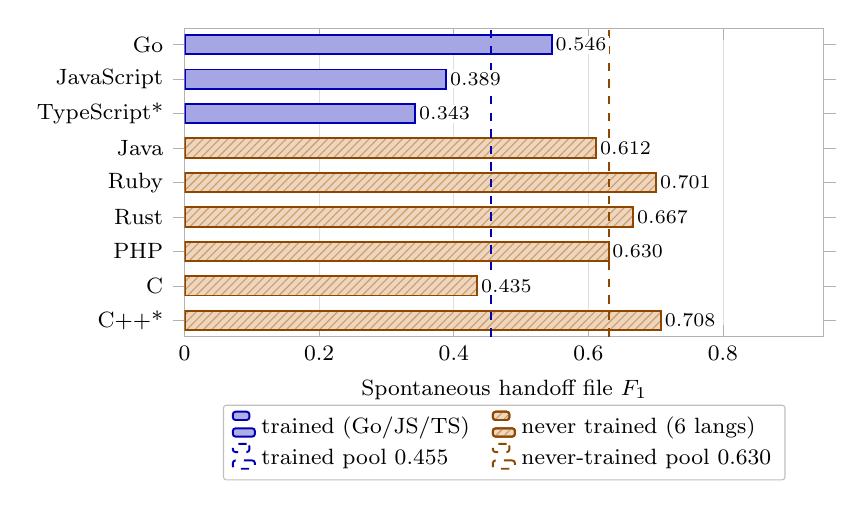
\begin{tikzpicture}
\begin{axis}[
  paperaxis,
  width=0.80\linewidth,
  height=5.5cm,
  xbar,
  bar width=7pt,
  xmin=0, xmax=0.95,
  xtick={0,0.2,0.4,0.6,0.8},
  xlabel={Spontaneous handoff file $F_1$},
  symbolic y coords={{Go},{JavaScript},{TypeScript*},
                     {Java},{Ruby},{Rust},{PHP},{C},{C++*}},
  ytick={{Go},{JavaScript},{TypeScript*},
         {Java},{Ruby},{Rust},{PHP},{C},{C++*}},
  y dir=reverse,
  enlarge y limits=0.06,
  xmajorgrids=true,
  nodes near coords,
  % white fill so the two dashed pool lines never run through a value label
  nodes near coords style={font=\scriptsize, fill=white, inner sep=1pt,
                           /pgf/number format/fixed,
                           /pgf/number format/fixed zerofill,
                           /pgf/number format/precision=3},
  legend style={at={(0.5,-0.22)}, anchor=north, legend columns=2,
                /tikz/every even column/.append style={column sep=6pt}},
  legend cell align=left,
]

% ---- trained pool: Go / JavaScript / TypeScript (solid) ----------------
\addplot[fill=cSys!35, draw=cSys, bar shift=0pt]
  coordinates {(0.546,{Go}) (0.389,{JavaScript}) (0.343,{TypeScript*})};
\addlegendentry{trained (Go/JS/TS)}

% ---- never-trained pool (hatched, so the split survives grayscale) -----
\addplot[fill=cFlash!25, draw=cFlash!80!black, bar shift=0pt,
         postaction={pattern=north east lines, pattern color=cFlash!60}]
  coordinates {(0.612,{Java}) (0.701,{Ruby}) (0.667,{Rust})
               (0.630,{PHP}) (0.435,{C}) (0.708,{C++*})};
\addlegendentry{never trained (6 langs)}

% ---- pooled aggregates: 0.455 (trained) and 0.630 (never-trained) ------
% x positions as axis fractions: 0.455/0.95 and 0.630/0.95.
\draw[dashed, cSys, line width=0.7pt]
  (rel axis cs:0.47895,0) -- (rel axis cs:0.47895,1);
\draw[dashed, cFlash!80!black, line width=0.7pt]
  (rel axis cs:0.66316,0) -- (rel axis cs:0.66316,1);
% the two dashed lines are identified in the legend rather than in-plot,
% where they would collide with the bar value labels.
\addlegendimage{dashed, cSys, line width=0.7pt}
\addlegendentry{trained pool 0.455}
\addlegendimage{dashed, cFlash!80!black, line width=0.7pt}
\addlegendentry{never-trained pool 0.630}

\end{axis}
\end{tikzpicture}
